\documentclass[border=10pt]{standalone}

\usepackage{tikz}
\usepackage{tikzsymbols}
\usetikzlibrary{calc,patterns,shapes.geometric}

\def\centerarc[#1](#2)(#3:#4:#5){\draw[#1] ($(#2)+({#5*cos(#3)},{#5*sin(#3)})$) arc (#3:#4:#5);}

\begin{document}
	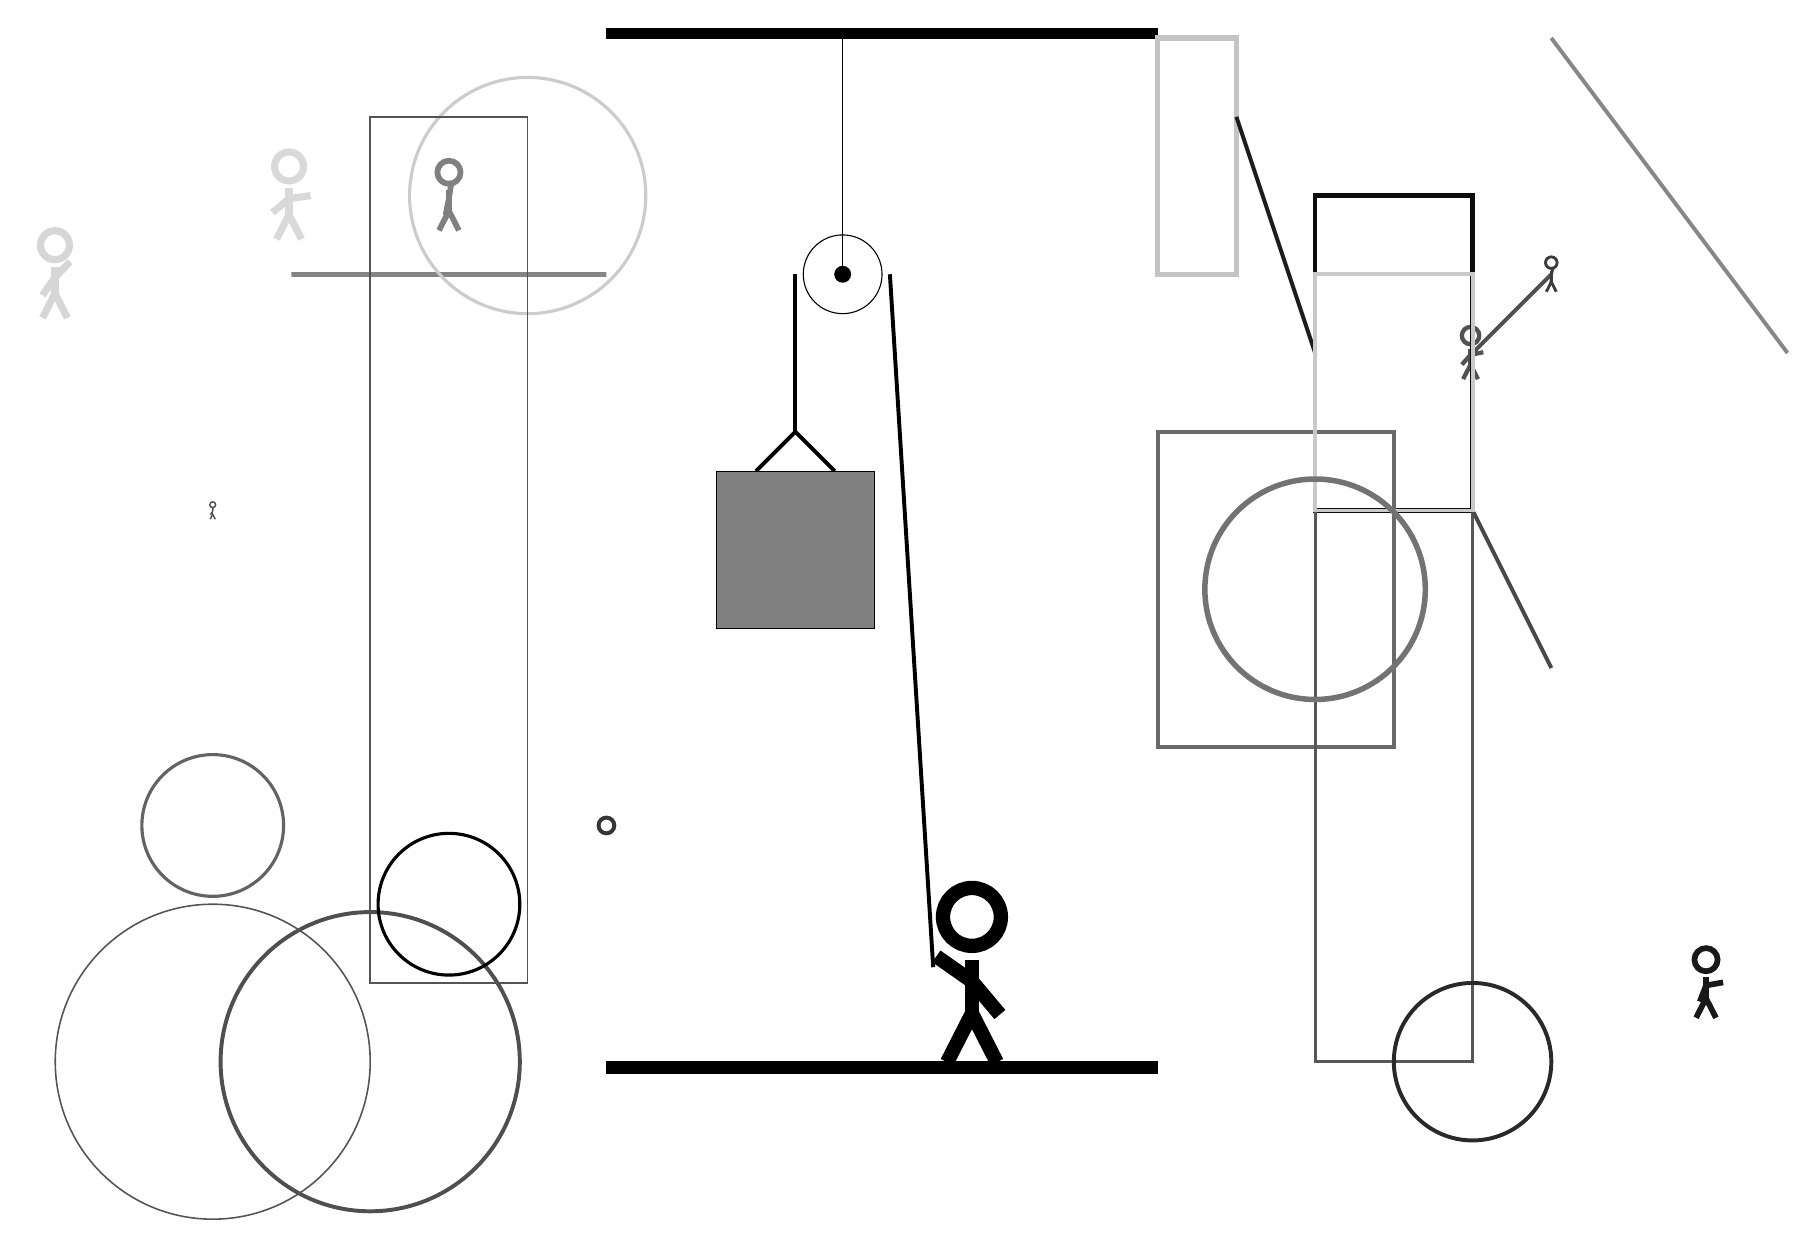
\begin{tikzpicture}
		%%%%% START %%%%%
		
		\draw[fill=black] (-2, 10) rectangle (5, 10.125);
		
		\draw (1, 7) circle (0.5);
		\draw[fill=black] (1, 7) circle (0.1);
		\draw (1, 10) -- (1, 7);
		
		\draw[line width=0.6mm, color=black!48] (-2, 7) rectangle (-6, 7);
		
		\draw [line width=0.5mm, color=black!69](-5, -3) circle (1.9);
		\draw [line width=0.4mm, color=black!61](-7, 0) circle (0.9);
		\node[line width=0.2mm, color=black!68] at (9, 6) {\Strichmaxerl[3][48][12]};
		
		\draw [line width=0.4mm, color=black!20](-3, 8) circle (1.5);
		\node[line width=0.3mm, color=black!15] at (-6, 8) {\Strichmaxerl[5][40][8]};
		\draw[line width=0.5mm, color=black!69](10, 7) -- (9, 6);
		\draw [line width=0.2mm, color=black!67](-7, -3) circle (2.0);
		\node[line width=0.7mm, color=black!90] at (12, -2) {\Strichmaxerl[4][69][10]};
		
		\draw[line width=0.6mm, color=black!95] (7, 4) rectangle (9, 8);
		\draw[line width=0.7mm, color=black!23] (6, 7) rectangle (5, 10);
		\draw[line width=0.5mm, color=black!59] (5, 5) rectangle (8, 1);
		\draw[line width=0.5mm, color=black!89](6, 9) -- (7, 6);
		
		\draw[line width=0.2mm, color=black!67] (-3, 9) rectangle (-5, -2);
		\draw[line width=0.4mm, color=black!66] (7, 4) rectangle (9, -3);
		\draw [line width=0.5mm, color=black!79](-2, 0) circle (0.1);
		\draw[line width=0.5mm, color=black!72](10, 2) -- (9, 4);
		
		\node[line width=0.7mm, color=black!77] at (10, 7) {\Strichmaxerl[2][88][79]};
		\draw[line width=0.4mm, color=black!54] (6, 7) rectangle (6, 7);
		
		\draw[line width=0.5mm, color=black!47](10, 10) -- (13, 6);
		\draw [line width=0.5mm, color=black!84](9, -3) circle (1.0);
		
		\draw[line width=0.5mm, color=black!21] (7, 4) rectangle (9, 7);
		
		\draw [line width=0.4mm, color=black!100](-4, -1) circle (0.9);
		\node[line width=0.7mm, color=black!50] at (-4, 8) {\Strichmaxerl[4][79][81]};
		\draw [line width=0.7mm, color=black!55](7, 3) circle (1.4);
		
		\node[line width=0.5mm, color=black!69] at (-7, 4) {\Strichmaxerl[1][58][86]};
		
		\node[line width=0.2mm, color=black!16] at (-9, 7) {\Strichmaxerl[5][55][46]};
		
		\draw[line width=0.5mm] (-0.1, 4.5) -- (0.4, 5.0) -- (0.9, 4.5);
		\draw[fill=black!50] (-0.6, 4.5) rectangle (1.4, 2.5);
		
		\draw[line width=0.5mm] (0.4, 7) -- (0.4, 5.0);
		\centerarc[line width=0.5mm](1, 7)(0:180:0.6);
		\draw[line width=0.5mm](1.6, 7) -- (2.15, -1.8);
		
		\node at (2.6, -1.9) {\Strichmaxerl[10][-35][-50]};
		
		\draw[fill=black] (-2, -3) rectangle (5, -3.15);
		
		%%%%% END %%%%%
	\end{tikzpicture}
\end{document}